\chapter{Martensitzerfall}

\section{Durchführung (TJ)}

Für eine weitere Wärmebehandlung wird untersucht, ob die Festigkeit der Legierung weiter steigt. Ein dritter Schritt ist wie im Three Step Short Time Duplex Anneal Behandlung geplant \cite{Morita.2005}. Das gebildete Martensit aus der vorherigen Behandlung soll partiell zerfallen. Das nadelförmige $\alpha'$ wandelt sich in $\alpha$ + $\beta$ Phase um. Hier passiert der Prozess im transformierten $\beta$ Phase, also zwischen den Lamellen Pakete. Damit soll sich eine weitere Verfeinerung der Struktur ergeben, die zu eine Festigkeitssteigerung erbringt.

Untersucht wird ob bei der Ti-6242 Legierung solch eine Behandlung auch erfolgreich ist. Die verwendeten Temperaturen werden nach einem Vergleich mit Paper für Ti-64 \cite{Morita.2005} ausgewählt. Die zwei Ti-6242 Legierung werden erstmals bei 580$^\circ$C für 8 bzw. 16 Minuten geglüht. Weiterhin wird beobachtet, ob es einen Unterschied bei einer höheren Temperatur gibt. Zwei weiteren Legierung werden bei 610$^\circ$C unter gleichen Bedingungen angelassen (Siehe Prinzip Bild). Damit der Legierung nicht wieder auf ihre Bimodales Gefüge zurückkehrt, werden keine Temperaturen ausgewählt die nah der $T_{\beta}$ befinden. Stattdessen werden Temperaturen auserwählt die um 600$^\circ$C liegen. Schon die kurzen Glühzeiten sind  ausgesucht worden, weil extrem kleinen Diffusionsvorgänge im Nanometerbereich (zwischen die $\alpha$ Lamellen) herrschen. Außerdem ist Martensit nur lokal in einigen Bereichen des Gefüges zu finden und wandelt auch nicht komplett in $\alpha$ + $\beta$ um.

Dadurch, dass hier keine vollständige Umwandlung zu sehen ist, soll es für wenige Minuten angelassen werden. Das Martensit zerfällt partiell. Falls es für eine zu lange Zeit geglüht wird, kommt es zu eine Vergröberung der Phase in transformiertes $\beta$. Dieses führt dann zu einen weicheren Gefüge.

\section{Ergebnisse (PH)}

Im dritten Schritt war der Zerfall des Martensits, dass vorher gebildet wurde, geplant. Dazu wurde die Probe aus Abbildung \ref{fig:abbildung-18} (983$^\circ$C/1h/AC + 950$^\circ$C/16min/WQ), die die ausgeprägtesten Martensitstrukturen aufwies, für die weiteren Schritte ausgewählt. 
Dafür wurden vier Proben für den dritten Wärmebehandlungsschritt festgelegt. Zwei Proben wurden bei 580$^\circ$C und unterschiedlichen Haltezeiten (8 und 16 min) wärmebehandelt. Die zwei verbliebenen wurden den gleichen Haltezeiten ausgesetzt, nur bei höher Temperatur (610$^\circ$C).

Die Analyse unter dem Lichtmikroskop ergab keine sichtbare Veränderung der Mikrostruktur zur dritten Probenreihe. Die Ergebnisse der weiteren Auswertung unter dem REM sind in den Abbildungen \ref{fig:abbildung-22} -- \ref{fig:abbildung-25} zusammengefasst.

\begin{figure}[h]
	\centering
	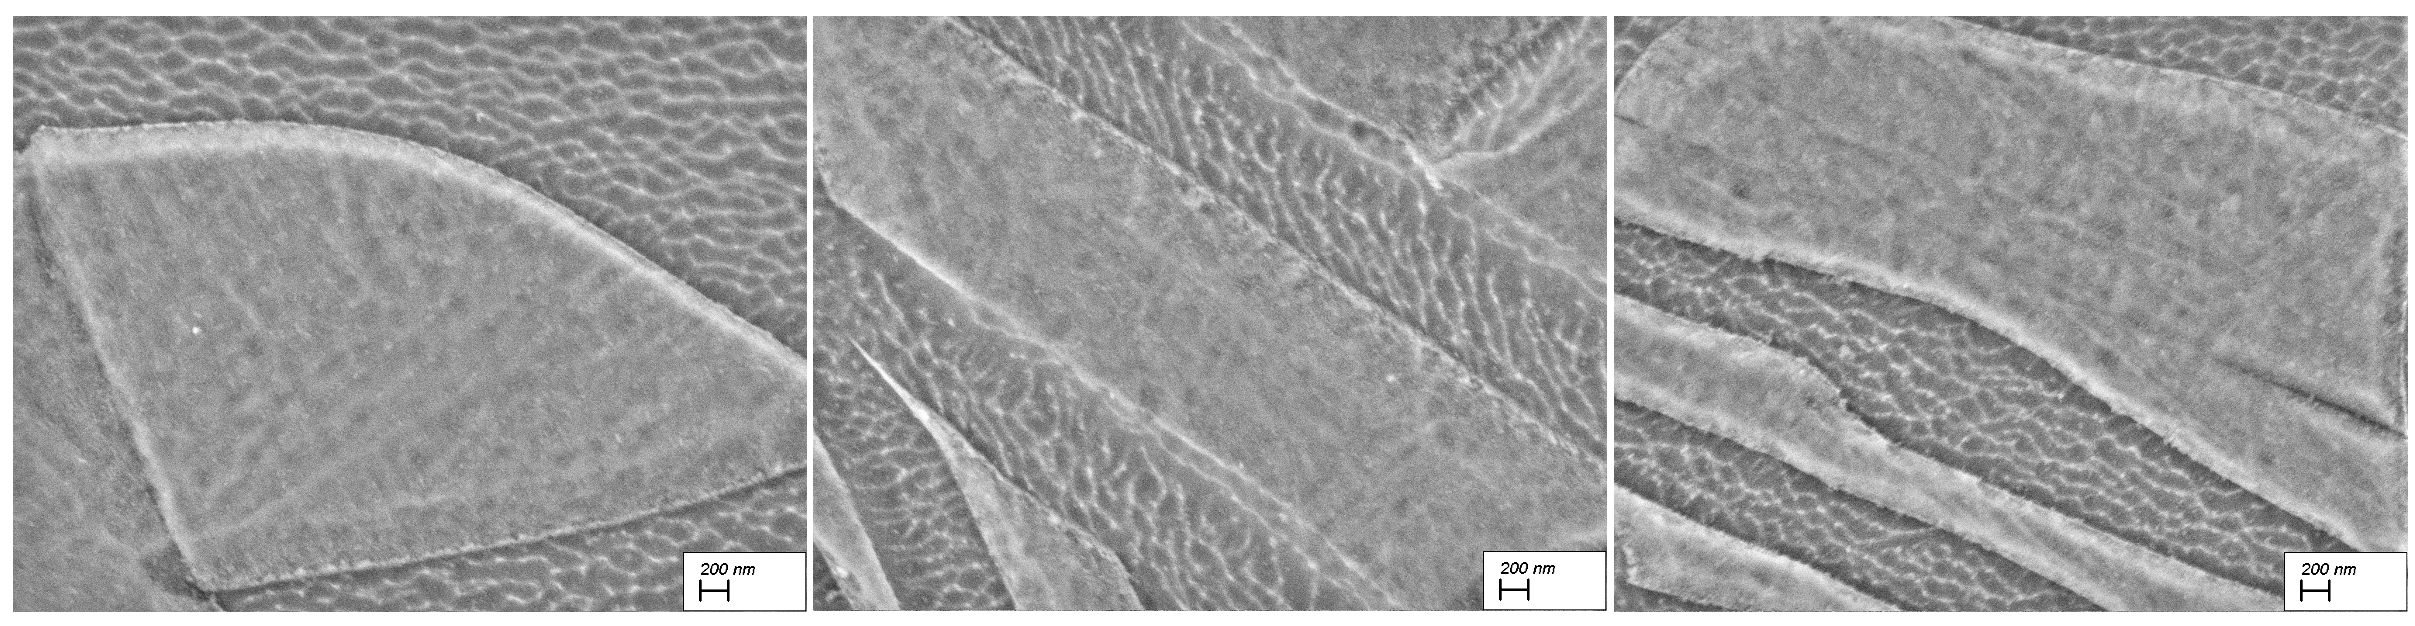
\includegraphics[width=1.0\linewidth]{./Bilder/Abbildung 22.png}
	\caption[Abbildung 22]{983$^\circ$C/1h/AC + 950$^\circ$C/16min/WQ + 580$^\circ$C/8min/AC, REM}
	\label{fig:abbildung-22}
\end{figure}

\begin{figure}[h]
	\centering
	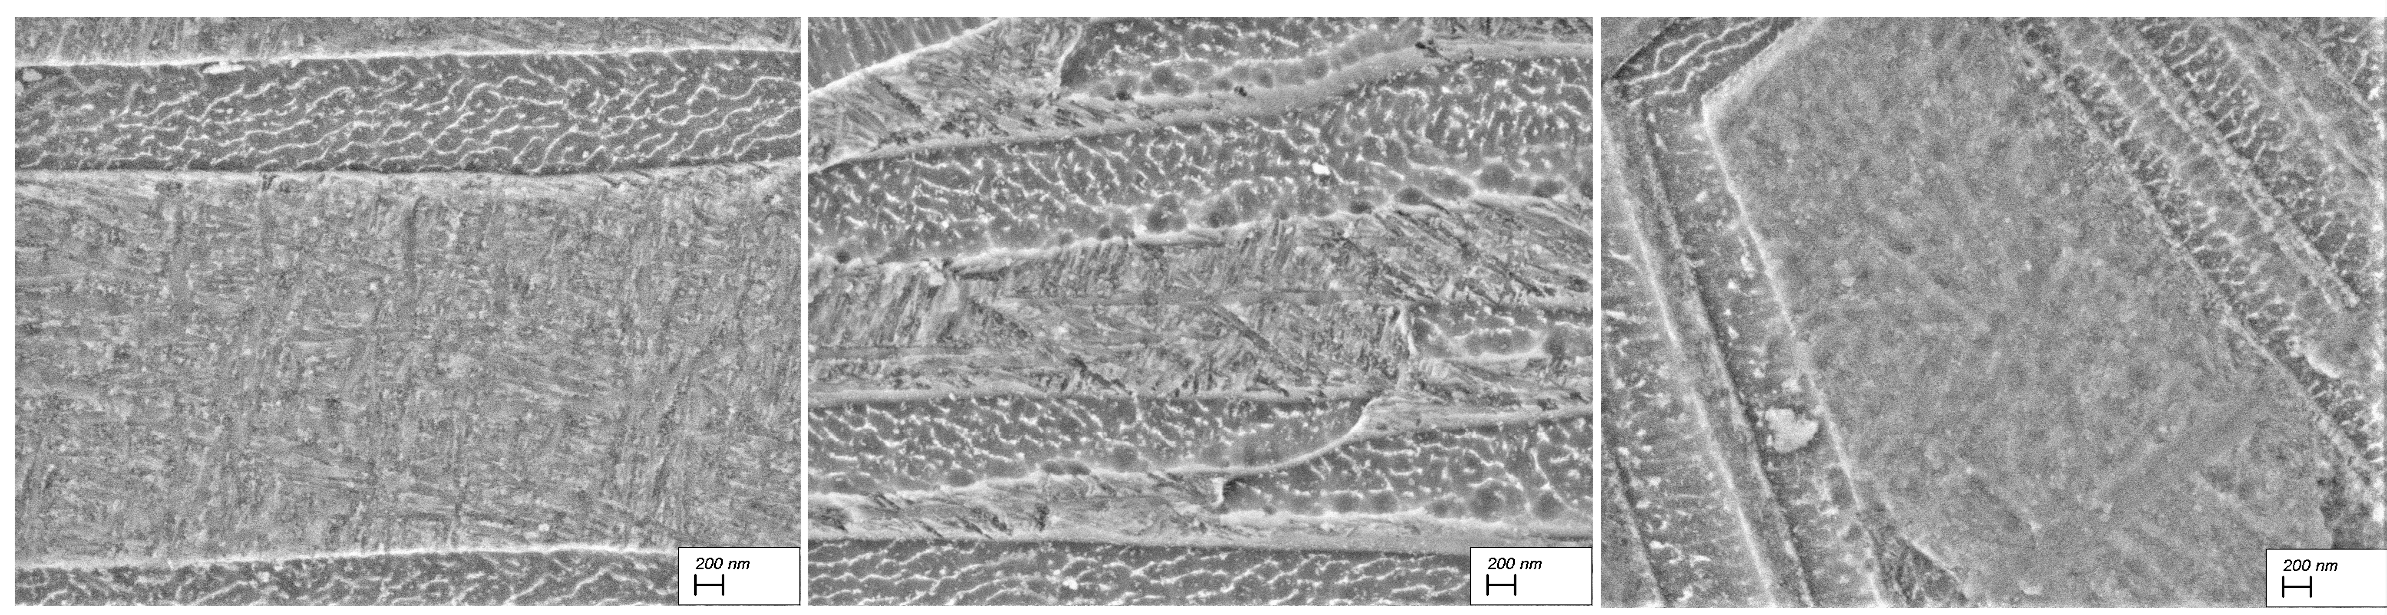
\includegraphics[width=1.0\linewidth]{./Bilder/Abbildung 23.png}
	\caption[Abbildung 23]{983$^\circ$C/1h/AC + 950$^\circ$C/16min/WQ + 580$^\circ$C/16min/AC, REM}
	\label{fig:abbildung-23}
\end{figure}

\begin{figure}[h]
	\centering
	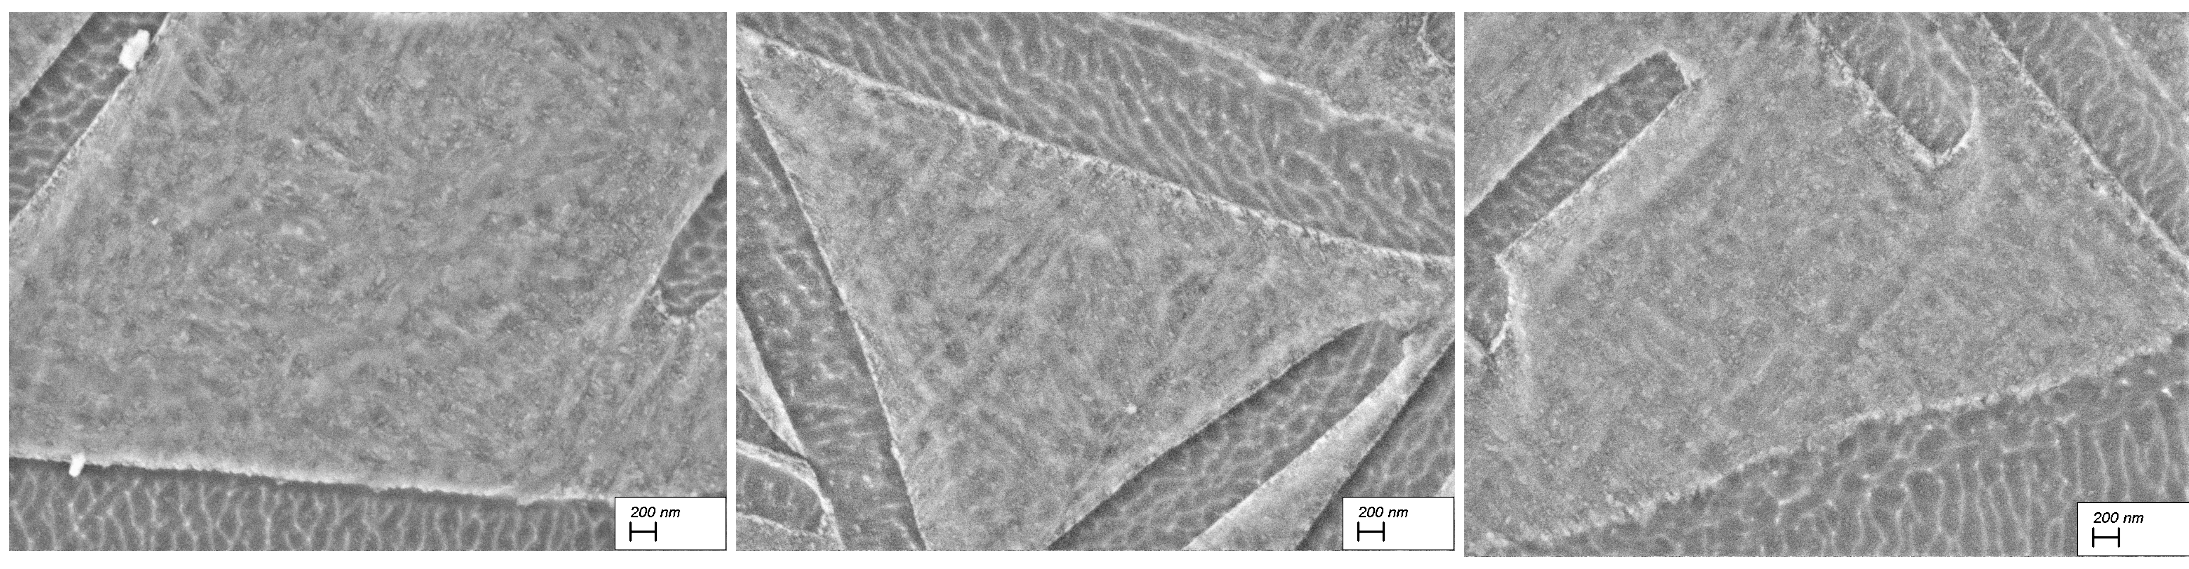
\includegraphics[width=1.0\linewidth]{./Bilder/Abbildung 24.png}
	\caption[Abbildung 24]{983$^\circ$C/1h/AC + 950$^\circ$C/16min/WQ + 610$^\circ$C/8min/AC, REM}
	\label{fig:abbildung-24}
\end{figure}

\begin{figure}[h]
	\centering
	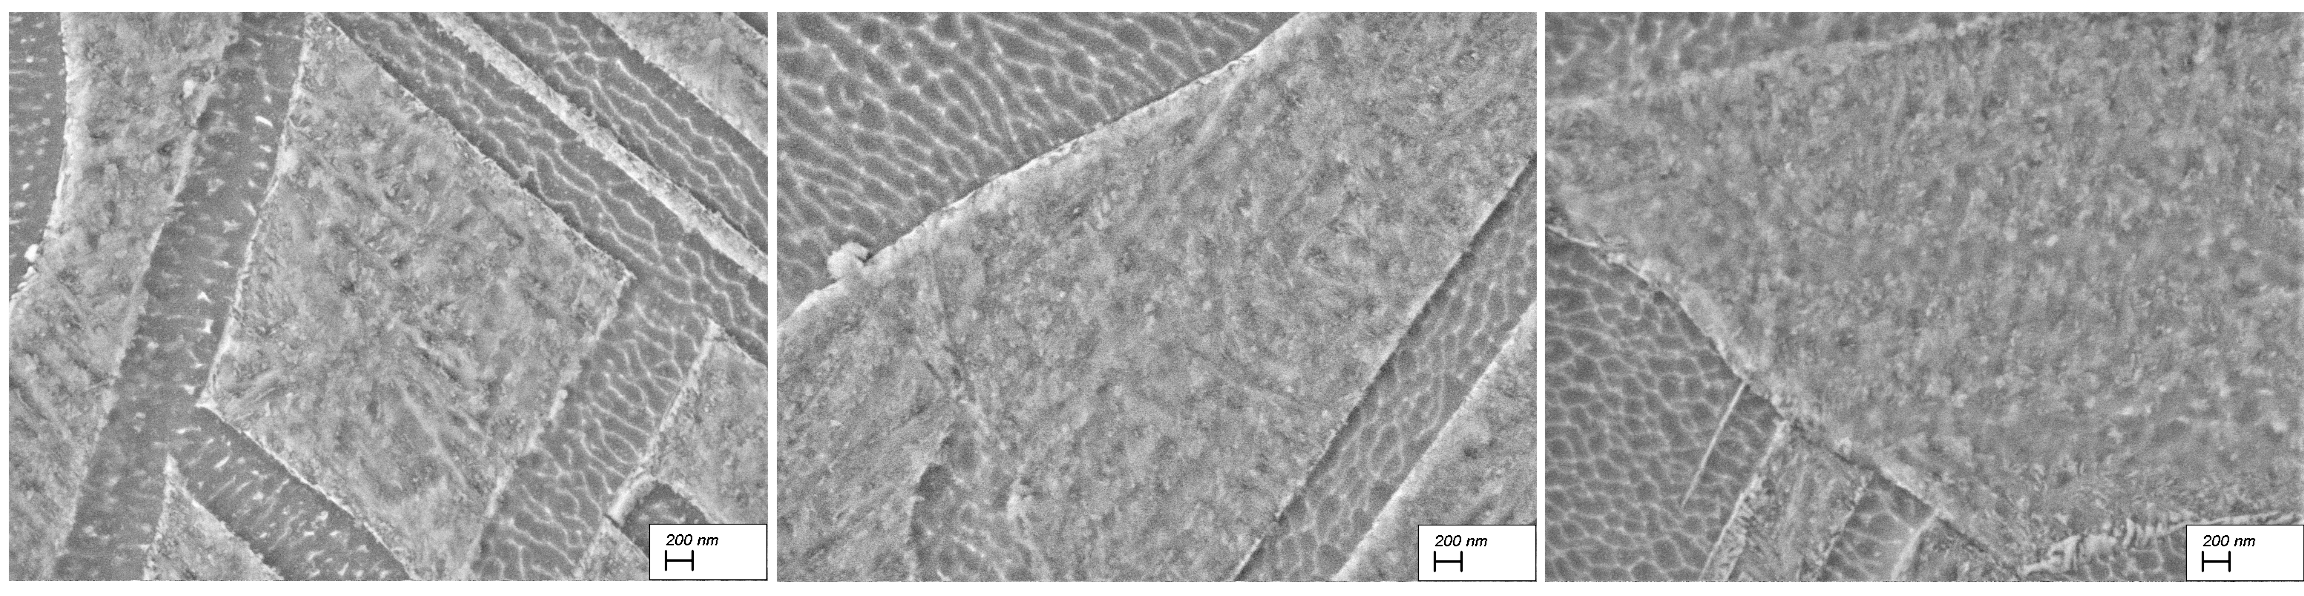
\includegraphics[width=1.0\linewidth]{./Bilder/Abbildung 25.png}
	\caption[Abbildung 25]{983$^\circ$C/1h/AC + 950$^\circ$C/16min/WQ + 610$^\circ$C/16min/AC, REM}
	\label{fig:abbildung-25}
\end{figure}

In den Abbildungen \ref{fig:abbildung-22} -- \ref{fig:abbildung-25} ist zu sehen, dass die Martensitstrukturen in der $\beta$-Phase zum größten Teil zerfallen sind. Es sind nur an vereinzelten Stellen der Proben noch ansatzweise Rückstände dieser Strukturen zu erkennen.

Die Härteprüfung zeigte im Gegensatz zur dritten Probenreihe eine sichtbare Härtesteigerung. Die Ergebnisse sind in Tabelle \ref{Tabelle 8} zusammengefasst.

\begin{table}[h]
	\centering
	\begin{tabular}{|c|c|}
		\hline 
		Probe & Härte in HV \\ 
		\hline 
		983$^\circ$C/1h/AC + 950$^\circ$C/16min/WQ + 580$^\circ$C/8min/AC & 393 \\ 
		\hline 
		983$^\circ$C/1h/AC + 950$^\circ$C/16min/WQ + 580$^\circ$C/16min/AC & 392 \\ 
		\hline 
		983$^\circ$C/1h/AC + 950$^\circ$C/16min/WQ + 610$^\circ$C/8min/AC & 399 \\ 
		\hline 
		983$^\circ$C/1h/AC + 950$^\circ$C/16min/WQ + 610$^\circ$C/16min/AC & 392 \\ 
		\hline 
	\end{tabular} 
	\caption{Ergebnisse der Härteprüfung nach dem Martensitzerfall}
	\label{Tabelle 8}
\end{table}

\section{Diskussion der Ergebnisse (TJ)}

Man sieht eine offensichtliche Erhöhung der Härte vom zweiten auf den dritten Schritt. Die beste Versuchsprobe aus der 2. Wärmebehandlung ist bei 950$^\circ$C /16 min/WQ mit 376 HV10 gemessen worden. Am dritten Schritt ist eine Härte von 393 bis 399 HV10 gemessen. Man beobachtet eine Erhöhung von 17 bis 23 HV10. Damit ist eine signifikante Steigerung der Härte in der Legierung stattgefunden. Eine Änderung der Gefüge ist im FE REM beobachtet. In dem transformierten $\beta$ Bereich sind keine Martensit-Strukturen in lokalen Stellen vorhanden und auch keine $\alpha$+$\beta$ Strukturen zu erkennen. Diese Veränderung der Gefügestruktur vom vorherigen Schritt führte zu eine Härtesteigerung. Wahrscheinlich ist dies auf den partiellen martensitischen Zerfall zurückzuführen.
\\Es ist eine Verfeinerung der Struktur festzustellen. Nach der dritter Schritt sind mehr Phasengrenzen erwartet, die zu eine feinere Gefüge führte und dabei die Härte gestiegen. Es sind sehr hohe Werte von 999HV10 zu Stande gekommen. Es hat sich gezeigt, dass bei alle Proben, die bei 580$^\circ$C und 610$^\circ$C geglüht wurden, Ähnlichen Werten haben. Allen Proben haben wahrscheinlich den Martensit zerfallen erreicht.
